% Options for packages loaded elsewhere
\PassOptionsToPackage{unicode}{hyperref}
\PassOptionsToPackage{hyphens}{url}
%
\documentclass[
  11pt,
  ignorenonframetext,
]{beamer}
\usepackage{pgfpages}
\setbeamertemplate{caption}[numbered]
\setbeamertemplate{caption label separator}{: }
\setbeamercolor{caption name}{fg=normal text.fg}
\beamertemplatenavigationsymbolsempty
% Prevent slide breaks in the middle of a paragraph
\widowpenalties 1 10000
\raggedbottom
\setbeamertemplate{part page}{
  \centering
  \begin{beamercolorbox}[sep=16pt,center]{part title}
    \usebeamerfont{part title}\insertpart\par
  \end{beamercolorbox}
}
\setbeamertemplate{section page}{
  \centering
  \begin{beamercolorbox}[sep=12pt,center]{part title}
    \usebeamerfont{section title}\insertsection\par
  \end{beamercolorbox}
}
\setbeamertemplate{subsection page}{
  \centering
  \begin{beamercolorbox}[sep=8pt,center]{part title}
    \usebeamerfont{subsection title}\insertsubsection\par
  \end{beamercolorbox}
}
\AtBeginPart{
  \frame{\partpage}
}
\AtBeginSection{
  \ifbibliography
  \else
    \frame{\sectionpage}
  \fi
}
\AtBeginSubsection{
  \frame{\subsectionpage}
}
\usepackage{amsmath,amssymb}
\usepackage{iftex}
\ifPDFTeX
  \usepackage[T1]{fontenc}
  \usepackage[utf8]{inputenc}
  \usepackage{textcomp} % provide euro and other symbols
\else % if luatex or xetex
  \usepackage{unicode-math} % this also loads fontspec
  \defaultfontfeatures{Scale=MatchLowercase}
  \defaultfontfeatures[\rmfamily]{Ligatures=TeX,Scale=1}
\fi
\usepackage{lmodern}
\usetheme[]{metropolis}
\ifPDFTeX\else
  % xetex/luatex font selection
\fi
% Use upquote if available, for straight quotes in verbatim environments
\IfFileExists{upquote.sty}{\usepackage{upquote}}{}
\IfFileExists{microtype.sty}{% use microtype if available
  \usepackage[]{microtype}
  \UseMicrotypeSet[protrusion]{basicmath} % disable protrusion for tt fonts
}{}
\makeatletter
\@ifundefined{KOMAClassName}{% if non-KOMA class
  \IfFileExists{parskip.sty}{%
    \usepackage{parskip}
  }{% else
    \setlength{\parindent}{0pt}
    \setlength{\parskip}{6pt plus 2pt minus 1pt}}
}{% if KOMA class
  \KOMAoptions{parskip=half}}
\makeatother
\usepackage{xcolor}
\newif\ifbibliography
\usepackage{color}
\usepackage{fancyvrb}
\newcommand{\VerbBar}{|}
\newcommand{\VERB}{\Verb[commandchars=\\\{\}]}
\DefineVerbatimEnvironment{Highlighting}{Verbatim}{commandchars=\\\{\}}
% Add ',fontsize=\small' for more characters per line
\newenvironment{Shaded}{}{}
\newcommand{\AlertTok}[1]{\textcolor[rgb]{1.00,0.00,0.00}{\textbf{#1}}}
\newcommand{\AnnotationTok}[1]{\textcolor[rgb]{0.38,0.63,0.69}{\textbf{\textit{#1}}}}
\newcommand{\AttributeTok}[1]{\textcolor[rgb]{0.49,0.56,0.16}{#1}}
\newcommand{\BaseNTok}[1]{\textcolor[rgb]{0.25,0.63,0.44}{#1}}
\newcommand{\BuiltInTok}[1]{\textcolor[rgb]{0.00,0.50,0.00}{#1}}
\newcommand{\CharTok}[1]{\textcolor[rgb]{0.25,0.44,0.63}{#1}}
\newcommand{\CommentTok}[1]{\textcolor[rgb]{0.38,0.63,0.69}{\textit{#1}}}
\newcommand{\CommentVarTok}[1]{\textcolor[rgb]{0.38,0.63,0.69}{\textbf{\textit{#1}}}}
\newcommand{\ConstantTok}[1]{\textcolor[rgb]{0.53,0.00,0.00}{#1}}
\newcommand{\ControlFlowTok}[1]{\textcolor[rgb]{0.00,0.44,0.13}{\textbf{#1}}}
\newcommand{\DataTypeTok}[1]{\textcolor[rgb]{0.56,0.13,0.00}{#1}}
\newcommand{\DecValTok}[1]{\textcolor[rgb]{0.25,0.63,0.44}{#1}}
\newcommand{\DocumentationTok}[1]{\textcolor[rgb]{0.73,0.13,0.13}{\textit{#1}}}
\newcommand{\ErrorTok}[1]{\textcolor[rgb]{1.00,0.00,0.00}{\textbf{#1}}}
\newcommand{\ExtensionTok}[1]{#1}
\newcommand{\FloatTok}[1]{\textcolor[rgb]{0.25,0.63,0.44}{#1}}
\newcommand{\FunctionTok}[1]{\textcolor[rgb]{0.02,0.16,0.49}{#1}}
\newcommand{\ImportTok}[1]{\textcolor[rgb]{0.00,0.50,0.00}{\textbf{#1}}}
\newcommand{\InformationTok}[1]{\textcolor[rgb]{0.38,0.63,0.69}{\textbf{\textit{#1}}}}
\newcommand{\KeywordTok}[1]{\textcolor[rgb]{0.00,0.44,0.13}{\textbf{#1}}}
\newcommand{\NormalTok}[1]{#1}
\newcommand{\OperatorTok}[1]{\textcolor[rgb]{0.40,0.40,0.40}{#1}}
\newcommand{\OtherTok}[1]{\textcolor[rgb]{0.00,0.44,0.13}{#1}}
\newcommand{\PreprocessorTok}[1]{\textcolor[rgb]{0.74,0.48,0.00}{#1}}
\newcommand{\RegionMarkerTok}[1]{#1}
\newcommand{\SpecialCharTok}[1]{\textcolor[rgb]{0.25,0.44,0.63}{#1}}
\newcommand{\SpecialStringTok}[1]{\textcolor[rgb]{0.73,0.40,0.53}{#1}}
\newcommand{\StringTok}[1]{\textcolor[rgb]{0.25,0.44,0.63}{#1}}
\newcommand{\VariableTok}[1]{\textcolor[rgb]{0.10,0.09,0.49}{#1}}
\newcommand{\VerbatimStringTok}[1]{\textcolor[rgb]{0.25,0.44,0.63}{#1}}
\newcommand{\WarningTok}[1]{\textcolor[rgb]{0.38,0.63,0.69}{\textbf{\textit{#1}}}}
\usepackage{longtable,booktabs,array}
\usepackage{calc} % for calculating minipage widths
\usepackage{caption}
% Make caption package work with longtable
\makeatletter
\def\fnum@table{\tablename~\thetable}
\makeatother
\usepackage{graphicx}
\makeatletter
\def\maxwidth{\ifdim\Gin@nat@width>\linewidth\linewidth\else\Gin@nat@width\fi}
\def\maxheight{\ifdim\Gin@nat@height>\textheight\textheight\else\Gin@nat@height\fi}
\makeatother
% Scale images if necessary, so that they will not overflow the page
% margins by default, and it is still possible to overwrite the defaults
% using explicit options in \includegraphics[width, height, ...]{}
\setkeys{Gin}{width=\maxwidth,height=\maxheight,keepaspectratio}
% Set default figure placement to htbp
\makeatletter
\def\fps@figure{htbp}
\makeatother
\setlength{\emergencystretch}{3em} % prevent overfull lines
\providecommand{\tightlist}{%
  \setlength{\itemsep}{0pt}\setlength{\parskip}{0pt}}
\setcounter{secnumdepth}{-\maxdimen} % remove section numbering
\ifLuaTeX
  \usepackage{selnolig}  % disable illegal ligatures
\fi
\IfFileExists{bookmark.sty}{\usepackage{bookmark}}{\usepackage{hyperref}}
\IfFileExists{xurl.sty}{\usepackage{xurl}}{} % add URL line breaks if available
\urlstyle{same}
\hypersetup{
  pdftitle={Biogeografía de islas},
  pdfauthor={Gerardo Martín},
  hidelinks,
  pdfcreator={LaTeX via pandoc}}

\title{Biogeografía de islas}
\subtitle{Modelos}
\author{Gerardo Martín}
\date{28-07-2023}

\begin{document}
\frame{\titlepage}

\hypertarget{intro}{%
\subsection{Intro}\label{intro}}

\begin{frame}{Intro}
\begin{itemize}
\item
  Biogeografía es el estudio del efecto de la geografía en la diversidad
  biológica

  \begin{itemize}
  \item
    Analizaremos el caso especial de las islas
  \item
    Isla puede ser porción de tierra rodeada de agua, fragmento de
    bosque rodeado de cultivo, un árbol separado de otros\ldots{}
  \end{itemize}
\item
  Modelos de metapoblaciones \(\rightarrow\) parches ocupados por
  poblaciones por una sola especie
\item
  Modelos de islas \(\rightarrow\) parches ocupados por varias especies
\end{itemize}
\end{frame}

\hypertarget{esquema-del-proceso}{%
\subsection{Esquema del proceso}\label{esquema-del-proceso}}

\begin{frame}{Esquema del proceso}
\begin{center}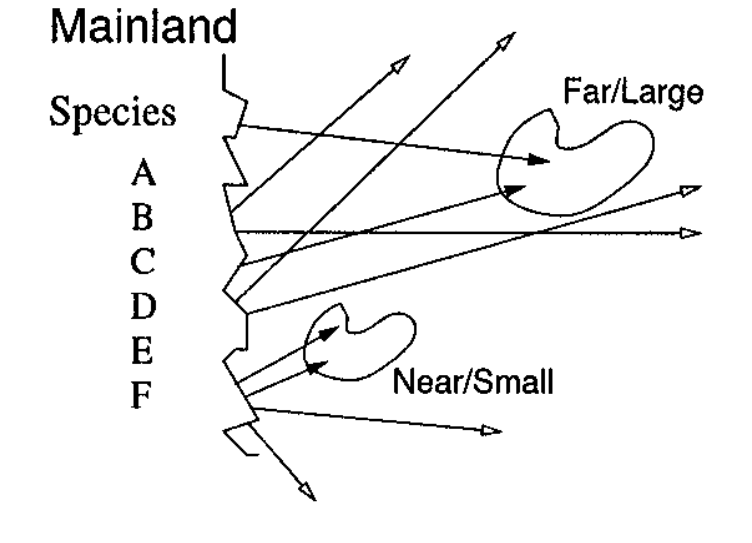
\includegraphics{Biogeografia/Islas} \end{center}
\end{frame}

\hypertarget{alternativas-tuxe9cnicas}{%
\subsection{Alternativas técnicas}\label{alternativas-tuxe9cnicas}}

\begin{frame}{Alternativas técnicas}
\begin{enumerate}
\item
  Representar movimiento de individuos desde continente

  \begin{enumerate}
  \tightlist
  \item
    Analizar frecuencia de llegada a las islas
  \end{enumerate}
\item
  Ignorar individuos \(\rightarrow\) representar número de especies como
  población

  \begin{enumerate}
  \tightlist
  \item
    Mac Arthur y Wilson 1967
  \end{enumerate}
\end{enumerate}
\end{frame}

\hypertarget{el-modelo-de-mac-arthur-y-wilson}{%
\subsection{El modelo de Mac Arthur y
Wilson}\label{el-modelo-de-mac-arthur-y-wilson}}

\begin{frame}{El modelo de Mac Arthur y Wilson}
\begin{enumerate}
\item
  Número de especies \(\rightarrow\) balance entre colonización y
  extinción
\item
  \(\forall\) spp tienen misma prob de llegar a isla
\item
  Sólo cuentan las colonizaciones, llegada de spp nuevas
\item
  Probabilidad de extinción es constante
\item
  Probabilidad de extinción de cualquier especie aumenta con el número
  de especies en isla
\end{enumerate}
\end{frame}

\hypertarget{el-modelo-de-mac-arthur-y-wilson-1967}{%
\subsection{El modelo de Mac Arthur y Wilson
(1967)}\label{el-modelo-de-mac-arthur-y-wilson-1967}}

\begin{frame}{El modelo de Mac Arthur y Wilson (1967)}
\begin{figure}

{\centering 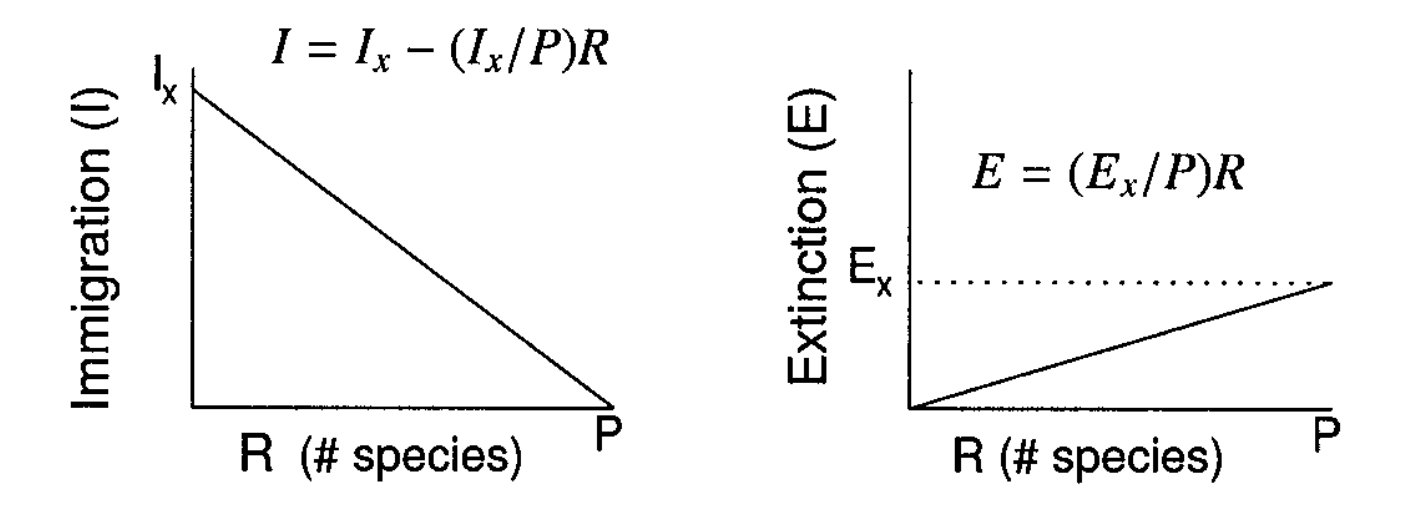
\includegraphics{Biogeografia/MacArthur} 

}

\caption{Relaciones cuantitativas entre inmigración, extinción, especies presentes y posibles.}\label{fig:unnamed-chunk-2}
\end{figure}
\end{frame}

\hypertarget{donde}{%
\subsection{Donde \ldots{}}\label{donde}}

\begin{frame}{Donde \ldots{}}
\begin{align}
I &= I_x - (I_x/P)R \\
E &= (E_x/P)R
\end{align}

\begin{itemize}
\item
  \(I =\) inmigración
\item
  \(E =\) extinción
\item
  \(P =\) número de especies que pueden colonizar la isla
\item
  \(R =\) número de especies que habitan la isla
\end{itemize}
\end{frame}

\hypertarget{section}{%
\subsection{\ldots{}}\label{section}}

\begin{frame}{\ldots{}}
\begin{itemize}
\item
  \(I_x\) es la tasa máxima de colonización
\item
  \(E_x\) es la tasa máxima de extinción
\end{itemize}

Por lo tanto el modelo completo es:

\[R_{t+1} = R_t + I_x - (I_x/P)R_t - (E_x/P)R_t\]
\end{frame}

\hypertarget{caracteruxedsticas-del-modelo-de-mac-arthur-y-wilson}{%
\subsection{Características del modelo de Mac Arthur y
Wilson}\label{caracteruxedsticas-del-modelo-de-mac-arthur-y-wilson}}

\begin{frame}{Características del modelo de Mac Arthur y Wilson}
\begin{itemize}
\item
  Tiempo discreto
\item
  Inmigración disminuye si hay pocas especies en \(P\)
\item
  Extinción aumenta si hay pocas especies en \(P\)
\end{itemize}
\end{frame}

\hypertarget{ejemplo-del-modelo-resuelto}{%
\subsection{Ejemplo del modelo
resuelto}\label{ejemplo-del-modelo-resuelto}}

\begin{frame}[fragile]{Ejemplo del modelo resuelto}
\begin{Shaded}
\begin{Highlighting}[]
\NormalTok{R }\OtherTok{\textless{}{-}} \FunctionTok{numeric}\NormalTok{(}\DecValTok{100}\NormalTok{); R[}\DecValTok{1}\NormalTok{] }\OtherTok{\textless{}{-}} \DecValTok{10}
\NormalTok{Ix }\OtherTok{\textless{}{-}} \DecValTok{1}\NormalTok{; Ex }\OtherTok{\textless{}{-}} \FloatTok{0.5}\NormalTok{; P }\OtherTok{\textless{}{-}} \DecValTok{20}
\ControlFlowTok{for}\NormalTok{(i }\ControlFlowTok{in} \DecValTok{2}\SpecialCharTok{:}\FunctionTok{length}\NormalTok{(R))\{}
\NormalTok{  R[i] }\OtherTok{\textless{}{-}}\NormalTok{ R[i}\DecValTok{{-}1}\NormalTok{] }\SpecialCharTok{+}\NormalTok{ Ix }\SpecialCharTok{{-}}\NormalTok{ (Ix}\SpecialCharTok{/}\NormalTok{P)}\SpecialCharTok{*}\NormalTok{R[i}\DecValTok{{-}1}\NormalTok{] }\SpecialCharTok{{-}}\NormalTok{ Ex}\SpecialCharTok{/}\NormalTok{P}\SpecialCharTok{*}\NormalTok{R[i}\DecValTok{{-}1}\NormalTok{]}
\NormalTok{\}}
\end{Highlighting}
\end{Shaded}
\end{frame}

\hypertarget{ejemplo-del-modelo-resuelto-1}{%
\subsection{Ejemplo del modelo
resuelto}\label{ejemplo-del-modelo-resuelto-1}}

\begin{frame}{Ejemplo del modelo resuelto}
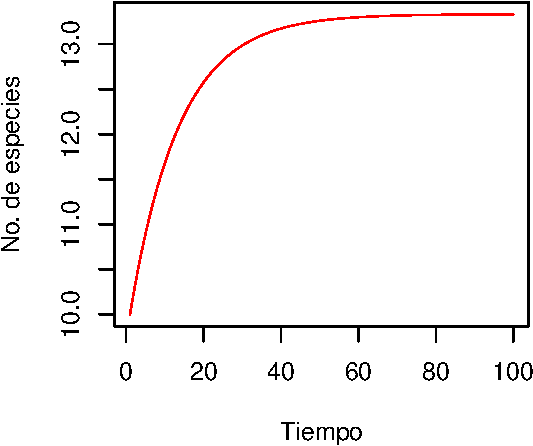
\includegraphics{Modelos-islas_files/figure-beamer/unnamed-chunk-4-1.pdf}
\end{frame}

\hypertarget{ejercicio}{%
\subsection{Ejercicio}\label{ejercicio}}

\begin{frame}{Ejercicio}
\begin{itemize}
\tightlist
\item
  Repetir la simulación con las siguientes combinaciones de parámetros
\end{itemize}

\begin{longtable}[]{@{}rrr@{}}
\toprule\noalign{}
Ix & Ex & P \\
\midrule\noalign{}
\endhead
0.75 & 0.75 & 20 \\
1.50 & 0.75 & 20 \\
0.75 & 1.25 & 20 \\
1.50 & 1.25 & 20 \\
0.75 & 0.75 & 40 \\
1.50 & 0.75 & 40 \\
0.75 & 1.25 & 40 \\
1.50 & 1.25 & 40 \\
\bottomrule\noalign{}
\end{longtable}
\end{frame}

\hypertarget{ejercicio-1}{%
\subsection{Ejercicio}\label{ejercicio-1}}

\begin{frame}{Ejercicio}
\begin{itemize}
\item
  ¿Qué pasa con el punto de equilibio cuando hay más especies en \(P\)?
\item
  ¿Cómo afectan \(I_x\) y \(E_x\) al número de especies en el conjunto
  de islas?
\end{itemize}
\end{frame}

\hypertarget{relaciuxf3n-entre-uxe1rea-distancia-y-especies}{%
\section{Relación entre área, distancia y
especies}\label{relaciuxf3n-entre-uxe1rea-distancia-y-especies}}

\hypertarget{concepto}{%
\subsection{Concepto}\label{concepto}}

\begin{frame}{Concepto}
\begin{itemize}
\item
  No.~spp disminuye con distancia de tierra
\item
  No.~spp aumenta con tamaño de isla
\item
  Se ha propuesto:
\end{itemize}

\[S = cA^z\]

\(S\) es el número de especies, \(c\) es una constante de grupo
taxonómico, \(z\) exponente sin dimensión
\end{frame}

\hypertarget{interpretaciuxf3n-de-paruxe1metros}{%
\subsection{Interpretación de
parámetros}\label{interpretaciuxf3n-de-paruxe1metros}}

\begin{frame}{Interpretación de parámetros}
\begin{itemize}
\item
  \(z \rightarrow\) tiene valores típicos de \(0.2-0.3\)
\item
  Indica que si área aumenta 10x número de especies aumenta 2x
\end{itemize}
\end{frame}

\hypertarget{evidencia}{%
\subsection{Evidencia}\label{evidencia}}

\begin{frame}{Evidencia}
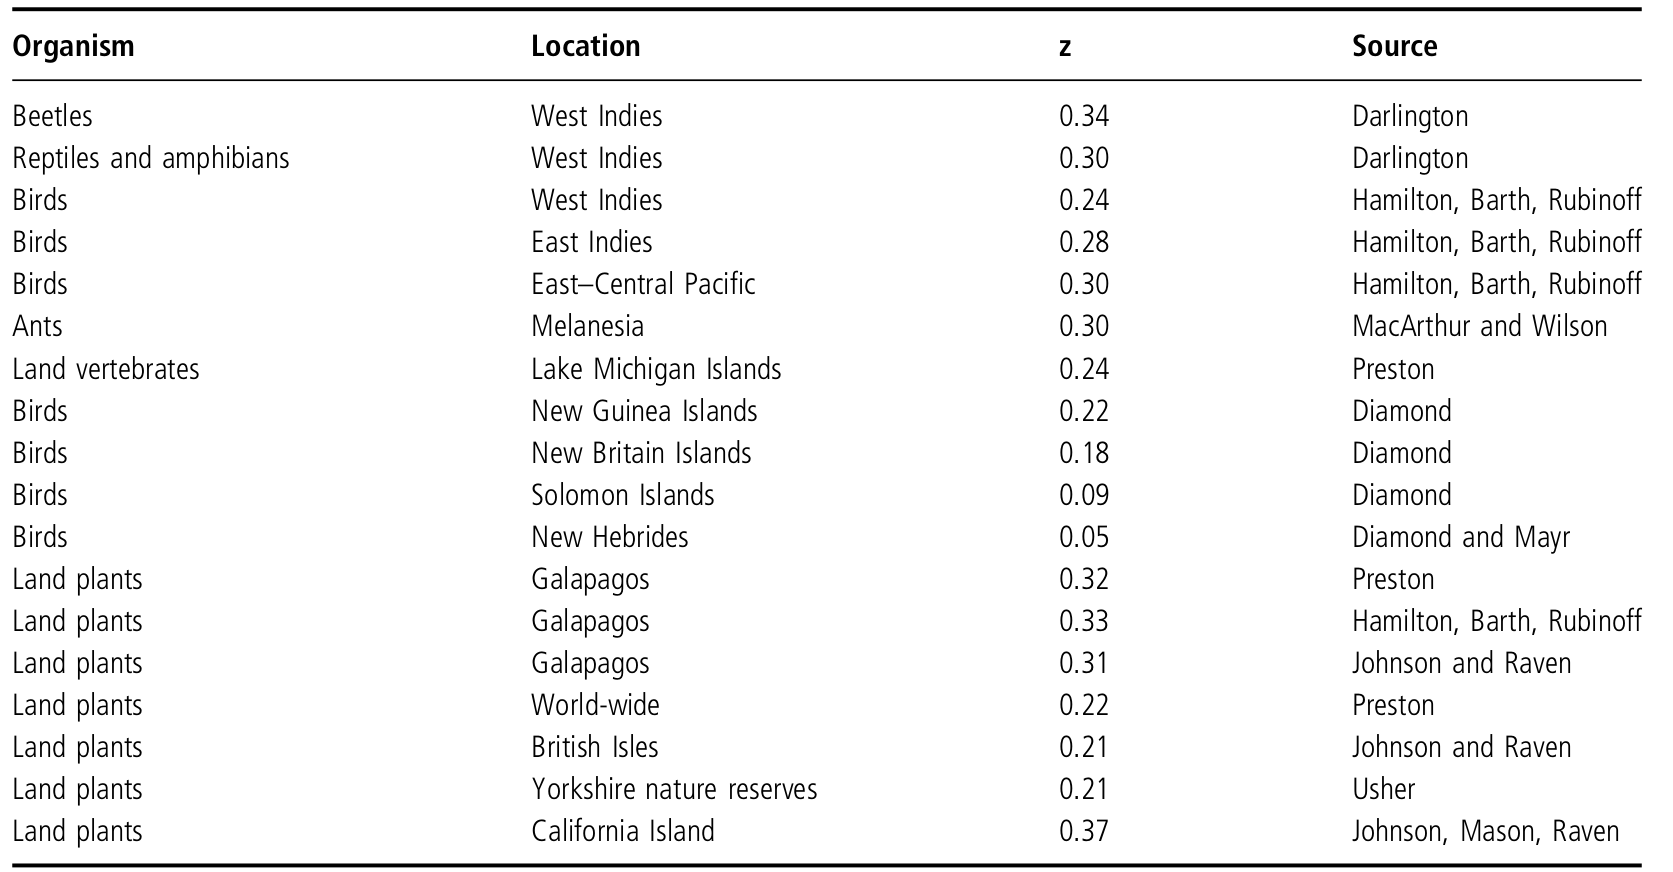
\includegraphics{Biogeografia/Spp-area.png}
\end{frame}

\hypertarget{mecanismos-bioluxf3gicos}{%
\subsection{Mecanismos biológicos}\label{mecanismos-bioluxf3gicos}}

\begin{frame}{Mecanismos biológicos}
\begin{enumerate}
\item
  Más especies pueden explotar nichos si el área es mayor
\item
  Áreas menores pueden albergar poblaciones más pequeñas
\item
  Extinciones pueden ocurrir por:

  \begin{itemize}
  \item
    Estocasticidad ambiental
  \item
    Emigración
  \item
    E\ldots?
  \end{itemize}
\end{enumerate}
\end{frame}

\hypertarget{supuestos}{%
\subsection{Supuestos}\label{supuestos}}

\begin{frame}{Supuestos}
\begin{enumerate}
\item
  La identidad de especies no importa
\item
  Todos los grupos taxonómicos se asumen igualmente probables

  \begin{itemize}
  \item
    Colonización
  \item
    Extinción
  \end{itemize}
\end{enumerate}
\end{frame}

\hypertarget{interacciuxf3n-entre-uxe1rea-y-distancia}{%
\subsection{Interacción entre área y
distancia}\label{interacciuxf3n-entre-uxe1rea-y-distancia}}

\begin{frame}{Interacción entre área y distancia}
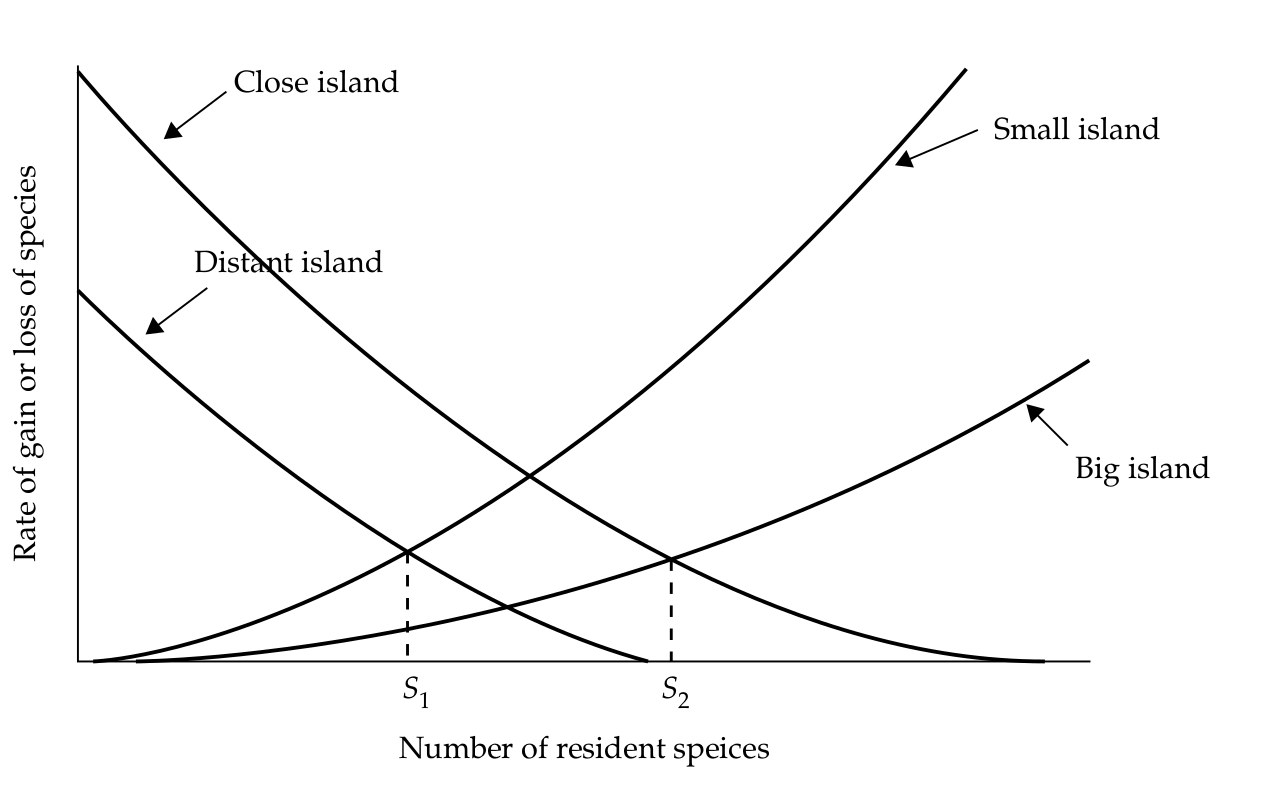
\includegraphics{Biogeografia/Distancia.Area.png}
\end{frame}

\hypertarget{supuestos-1}{%
\subsection{Supuestos}\label{supuestos-1}}

\begin{frame}{Supuestos}
\(A\) (área) es equivalente a \(N\) (número de especies)
\end{frame}

\end{document}
